\documentclass[12pt]{article}

% Specify how big is going to be the paper margins.
\usepackage[a4paper, margin=1in]{geometry}

% amsmath: Add useful commans like aligh and gather.
% amsfonts: Add useful fonts like \mathbb{R}.
% amssymb: Add useful symbles like \therefore (needs amsfonts to work).
\usepackage{amsmath, amsfonts, amssymb}

% Makes the use of colors possible.
\usepackage{xcolor}

\definecolor{color1}{HTML}{0e4a7a}
\definecolor{color2}{HTML}{1282d6}
\definecolor{color3}{HTML}{7ac1ff}

% Add Latin Modern Fonts like Sans-serif and Roman.
\usepackage{lmodern}

% Makes header and footer configurable.
\usepackage{fancyhdr}

% Makes the use of colored and configured tables possible
\usepackage[most]{tcolorbox}

% Add commands to specify theorems like \newtheorem{x}{y}.
\usepackage{amsthm}

% Enables enumeration of items.
\usepackage{enumitem}

% Enables adding images.
\usepackage{graphicx}

% Enables cool hyper references.
\usepackage[colorlinks=true, linkcolor=color2, urlcolor=color2, citecolor=color2]{hyperref}

\title{\sffamily\bfseries{Soluções OMpD 2022 N2 Fase 1}}
\author{Samuel de Araújo Brandão}
\date{5 de Setembro de 2025}

\pagestyle{fancy}
\fancyhf{}

\fancyhead[L]{\sffamily\bfseries{Soluções OMpD 2022 N2 Fase 1}}
\fancyhead[R]{\textcolor{color2}{Samuel Brandão}, 5 de Setembro de 2025}
\fancyfoot[C]{\thepage}
\setlength{\headheight}{14.5pt}

\tcbset{
  statementbox/.style = {
    enhanced,
    width=\textwidth,
    title={Enunciado},
    title filled,
    fonttitle=\sffamily\bfseries,
    coltitle=white,
    colbacktitle=color1,
    colback=white,
    colframe=color1,
    boxrule=1pt,
    arc=2mm,
    boxsep=2pt,
  }
}

\tcbset{
  theorembox/.style = {
    enhanced,
    width=\textwidth,
    colback=white,
    colframe=color1,
    boxrule=1pt,
    arc=2mm,
    boxsep=2pt
  }
}

\tcbset{
  lemmabox/.style = {
    enhanced,
    width=\textwidth,
    colback=white,
    colframe=color2,
    boxrule=1pt,
    arc=2mm,
    boxsep=2pt
  }
}

\renewcommand*\contentsname{\textsf{Conteúdos}}
\newcommand{\kb}[1]{\left\lfloor #1 \right\rfloor}

\begin{document}
  \maketitle
  Uma coleção de soluções para a \textbf{OMpD 2022 Nível 2 Fase 1}, inspirada no estilo de Evan Chen.
  Pode-se encontrar todos os problemas \textbf{\href{https://drive.google.com/file/d/1hwuCdi4SfUY-Gf1hCqBaIu7lwpr1JyxA/view}
  {aqui}} e as respostas oficiais \textbf{\href{https://drive.google.com/file/d/1epNXf5htopJSNVTkVXZBUBZU6akjIYoy/view}{aqui}}.

  Todas as soluções foram inteiramente escritas por mim, enquanto me preparava para a
  International Mathematical Olympiad (IMO).

  Caso encontre algum erro ou tiver sugestões ou comentários, sinta-se a vontade 
  para entrar em contato!

  \tableofcontents

  \clearpage

  \section{\textsf{Problemas}}
    \begin{enumerate}[label=\textbf{{\arabic*.}}]
      \item Qual o valor de $(-1)^{1^1} + (-1)^{2^2} + (-1)^{3^3} + \cdots + (-1)^{2022^{2022}}$?

(A) 2022 (B) 1 (C) -1 (D) -2022 (E) 0

\item Ana pensou em um número de dois dígitos $N$, onde o último dígito de $N$ é $7$. Ela somou os dígitos de $4N$ e obteve soma $13$. Qual o primeiro dígito de $N$?

(A) 3 (B) 6 (C) 7 (D) 8 (E) 9

\item Temos $33$ chocolates e colocamos cada um deles em uma dentre $7$ caixas (algumas caixas podem ficar vazias). É possível afirmar que:

\begin{enumerate}
\item[(A)] Existe uma caixa com pelo menos $6$ chocolates
\item[(B)] Existe uma caixa com no máximo $3$ chocolates
\item[(C)] Existe uma caixa com um número par de chocolates
\item[(D)] Existe uma caixa com um número ímpar de chocolates
\item[(E)] Existem duas caixas com o mesmo número de chocolates
\end{enumerate}

\item Sabendo que $ABCD$ é um retângulo e que $E$, $F$ são os pontos médios de $\overline{AB}$ e $\overline{CD}$, respectivamente, qual a porcentagem da área do retângulo corresponde à área hachurada?

  \begin{center}
  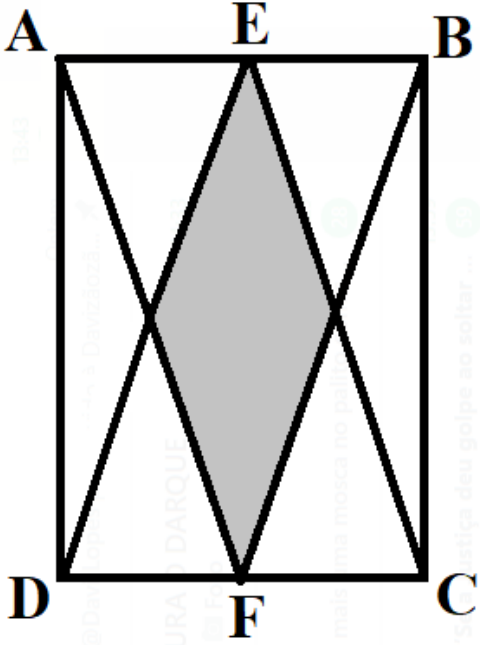
\includegraphics[width=0.25\textwidth]{first.png}
\end{center}


(A) 5\% (B) 10\% (C) 15\% (D) 20\% (E) 25\%

\item Na figura abaixo, os polígonos $ABCD$ e $ACEF$ são quadrados. Se $AB=1$, quanto é a medida do segmento $BE$?

  \begin{center}
  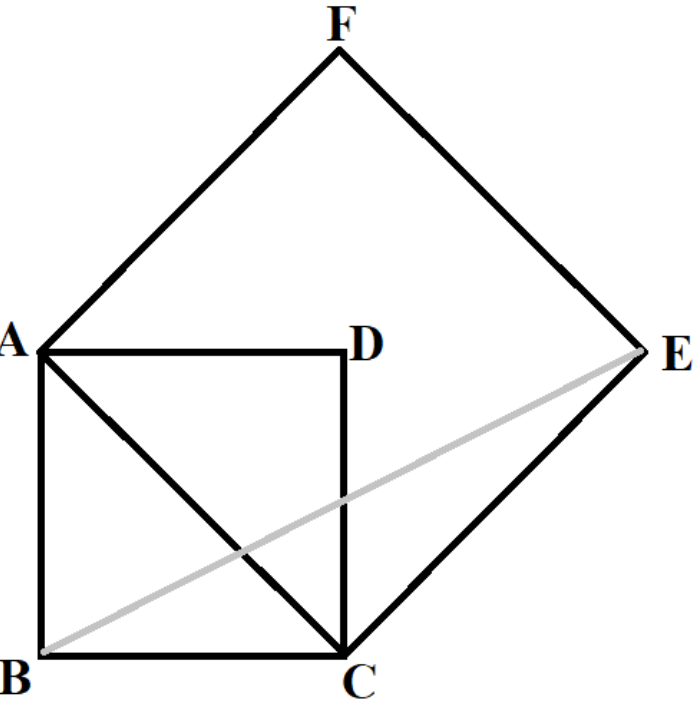
\includegraphics[width=0.2\textwidth]{second.png}
\end{center}


(A) $\sqrt{2}$ (B) $\sqrt{3}$ (C) $\sqrt{5}$ (D) $2\sqrt{2}$ (E) $2\sqrt{3}$

\item Qual o resto da divisão de $113333 + 331111$ por $7$?

(A) 0 (B) 1 (C) 3 (D) 5 (E) 6

\item Uma loja de computadores teve a seguinte ideia pensando na “Black Friday”: no mês de outubro, aumentou o valor dos computadores em $(5p)\%$ em relação a setembro, e no mês de novembro, reduziu o valor dos mesmos em $(4p)\%$ em relação a outubro. Sabe-se que o preço do computador é o mesmo em setembro e novembro (que novidade...). Qual é o valor de $p$?

(a) 5 (B) 8 (C) 10 (D) 12 (E) 15

\item Dizemos que um inteiro positivo é avizinhado se a diferença entre quaisquer dois de seus dígitos consecutivos é sempre igual a $1$. Por exemplo, $123456$, $987654$ e $45656765$ são avizinhados. Quantos são os inteiros entre $500{.}000$ e $600{.}000$ que são avizinhados?

(A) 8 (B) 10 (C) 31 (D) 32 (E) 64

\item De quantas maneiras podemos colocar $5$ garotas em fila, sendo $3$ delas Ana, Beatriz e Carla, de modo que Ana fique entre Beatriz e Carla?

(A) 6 (B) 20 (C) 30 (D) 40 (E) 60

\item Uma cidade euclidiana possui $2$ pontos turísticos $A$ e $B$, ligados por uma linha reta de $420$ metros de comprimento. Ana e Beatriz partem, do ponto $A$, em linha reta, em direção ao ponto $B$, com velocidades constantes de $5$ metros por segundo e $3$ metros por segundo, respectivamente. Enquanto isso, Carla parte do ponto $B$, em linha reta, em direção ao ponto $A$, com velocidade constante de $3$ metros por segundo. Sabendo que as $3$ garotas partem simultaneamente, quanto tempo após a partida Carla estará novamente a uma mesma distância de Ana e Beatriz?

(A) 30 segundos (B) 40 segundos (C) 50 segundos (D) 60 segundos (E) 70 segundos

\item No reticulado a seguir, a distância entre quaisquer dois pontos adjacentes na horizontal ou na vertical é igual a $1$ cm. Qual é a área, em cm$^{2}$, da região hachurada?

  \begin{center}
  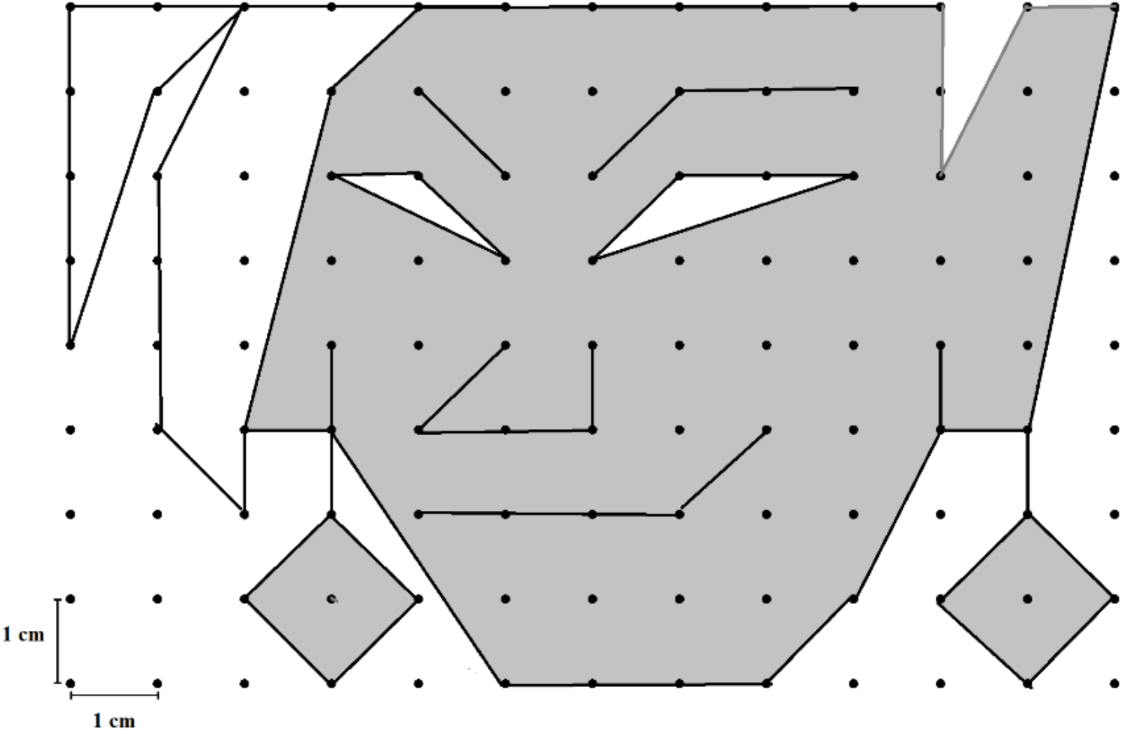
\includegraphics[width=0.5\textwidth]{third.png}
\end{center}


(A) 60 (B) 61 (C) 62 (D) 63 (E) 64

\item Sabe-se que o número $\underbrace{111\ldots 11}_{k\ \text{1’s}}$ é múltiplo de $17$, onde $k$ é um inteiro positivo. Qual é o menor valor possível de $k$?

(A) 4 (B) 11 (C) 16 (D) 18 (E) 34

\item De quantos modos podemos pintar as $5$ regiões da figura abaixo, usando em cada região uma dentre as cores preto, amarelo, rosa, azul e vermelho, de modo que regiões vizinhas tenham cores diferentes? \\
Observação: não é obrigatório que todas as $5$ cores sejam usadas na pintura.


  \begin{center}
  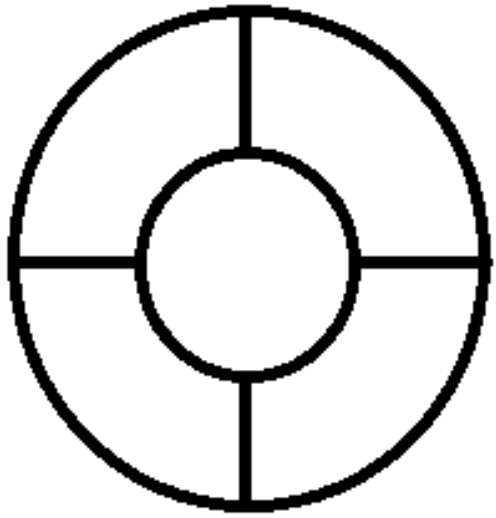
\includegraphics[width=0.25\textwidth]{fourth.png}
\end{center}


(A) 120 (B) 240 (C) 420 (D) 540 (E) 1280

\item Numa sala de aula, a quantidade de meninos é o dobro da quantidade de meninas. Certa vez, foi aplicada uma prova de matemática, e nessa prova a média dos meninos foi $7,4$ enquanto a média das meninas foi $8,6$. Qual foi a média das notas dos alunos da sala?

(A) 7,6 (B) 7,8 (C) 8 (D) 8,2 (E) 8,4

\item No triângulo $ABC$, temos $AB=2AC$. Sejam $D$, $E$ pontos em $\overline{AB}$, $\overline{BC}$, respectivamente, tais que $\angle BAE=\angle ACD$. Seja $F$ a interseção dos segmentos $\overline{AE}$ e $\overline{CD}$, e suponha que o triângulo $CFE$ é equilátero. Qual é a medida do ângulo $\angle ACB$?

(A) $60^\circ$ (B) $75^\circ$ (C) $90^\circ$ (D) $105^\circ$ (E) $120^\circ$

\item Para cada inteiro positivo $n$, sejam: \\
$T_n = 1 + 2 + \cdots + n$ \\
$P_n = \left(\dfrac{T_2}{T_2 - 1}\right)\left(\dfrac{T_3}{T_3 - 1}\right)\cdots\left(\dfrac{T_n}{T_n - 1}\right)$ \\
Qual é a alternativa mais próxima do valor numérico de $P_{2022}$?

(A) 2,90 (B) 2,93 (C) 2,96 (D) 2,99 (E) 3,02

\item Dizemos que um número inteiro é um “Matemático por Diversão” se ele pode ser escrito como a diferença de $2$ quadrados perfeitos não nulos. Por exemplo, $3$ é Matemático por Diversão, pois $3=2^2-1^2$. Quantos são os inteiros positivos, que não excedem $2022$, que são Matemáticos por Diversão?

(A) 506 (B) 507 (C) 1514 (D) 1516 (E) 2020

\item Seja $M=3318084147$. Qual dos números abaixo é um quadrado perfeito?

(A) $M$ (B) $3M$ (C) $5M$ (D) $7M$ (E) $11M$

\item Sejam $x$, $y$ números reais positivos tais que $x^2+y^2=7$ e $x^3+y^3=18$. Quanto vale $x^4+y^4$?

(A) 25 (B) 29 (C) 31 (D) 47 (E) 49

\item Duas circunferências, de raios $3$ e $4$, se cortam em dois pontos, sendo $Q$ um desses pontos. Traçam-se as tangentes externas comuns às duas circunferências. As duas tangentes se cortam em $P$ e uma dessas tangentes tangencia as circunferências nos pontos $A$ e $B$, conforme a figura abaixo: \\
Se $AB=6$, quanto vale $PQ$?

  \begin{center}
  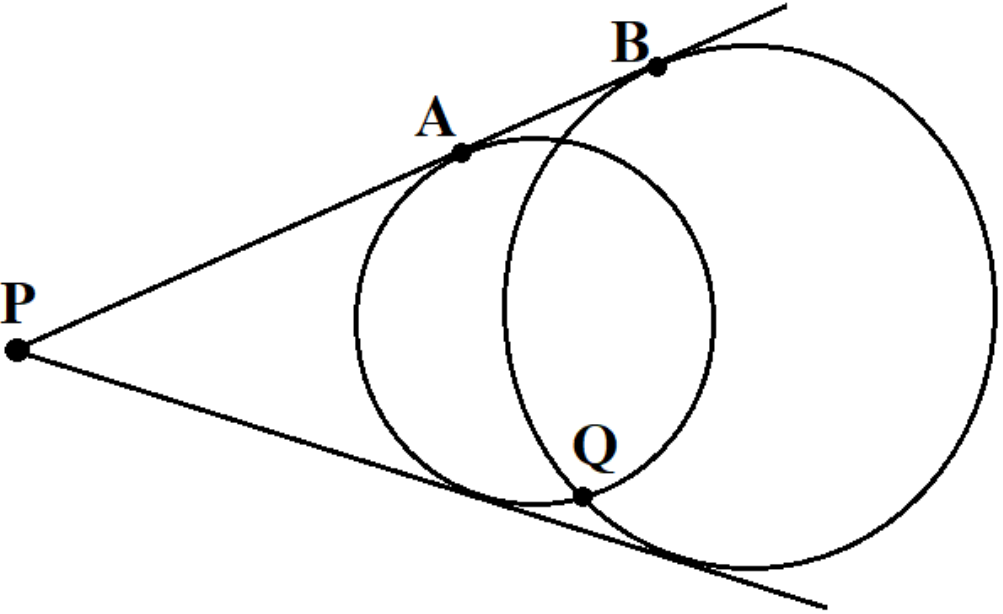
\includegraphics[width=0.25\textwidth]{fifth.png}
\end{center}


(A) 12 (B) $12\sqrt{3}$ (C) 21 (D) $21\sqrt{3}$ (E) 15

    \end{enumerate}

  \clearpage

  \section{\textsf{Soluções}}
\subsection{Problema 1}
\begin{tcolorbox}[statementbox]
      Qual o valor de $(-1)^{1^1} + (-1)^{2^2} + (-1)^{3^3} + \cdots + (-1)^{2022^{2022}}$?

(A) 2022 (B) 1 (C) -1 (D) -2022 (E) 0
\end{tcolorbox}
\clearpage

\subsection{Problema 2}
\begin{tcolorbox}[statementbox]
Ana pensou em um número de dois dígitos $N$, onde o último dígito de $N$ é $7$. Ela somou os dígitos de $4N$ e obteve soma $13$. Qual o primeiro dígito de $N$?

(A) 3 (B) 6 (C) 7 (D) 8 (E) 9
\end{tcolorbox}
\clearpage

\subsection{Problema 3}
\begin{tcolorbox}[statementbox]
Temos $33$ chocolates e colocamos cada um deles em uma dentre $7$ caixas (algumas caixas podem ficar vazias). É possível afirmar que:

\begin{enumerate}
\item[(A)] Existe uma caixa com pelo menos $6$ chocolates
\item[(B)] Existe uma caixa com no máximo $3$ chocolates
\item[(C)] Existe uma caixa com um número par de chocolates
\item[(D)] Existe uma caixa com um número ímpar de chocolates
\item[(E)] Existem duas caixas com o mesmo número de chocolates
\end{enumerate}
\end{tcolorbox}
\clearpage

\subsection{Problema 4}
\begin{tcolorbox}[statementbox]
Sabendo que $ABCD$ é um retângulo e que $E$, $F$ são os pontos médios de $\overline{AB}$ e $\overline{CD}$, respectivamente, qual a porcentagem da área do retângulo corresponde à área hachurada?

  \begin{center}
  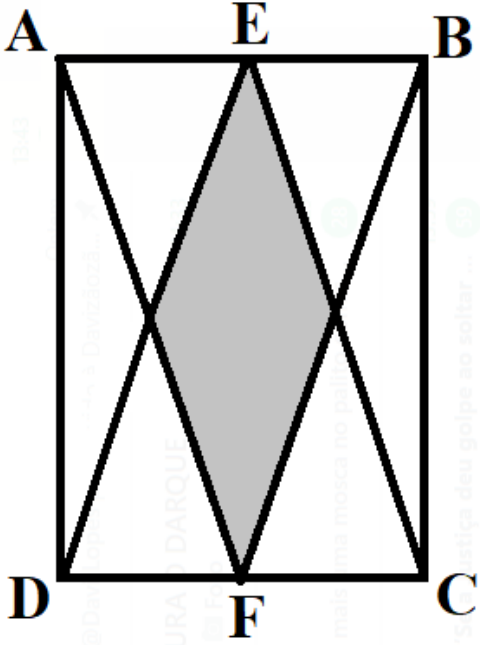
\includegraphics[width=0.25\textwidth]{first.png}
\end{center}


(A) 5\% (B) 10\% (C) 15\% (D) 20\% (E) 25\%
\end{tcolorbox}
\clearpage

\subsection{Problema 5}
\begin{tcolorbox}[statementbox]
Na figura abaixo, os polígonos $ABCD$ e $ACEF$ são quadrados. Se $AB=1$, quanto é a medida do segmento $BE$?

  \begin{center}
  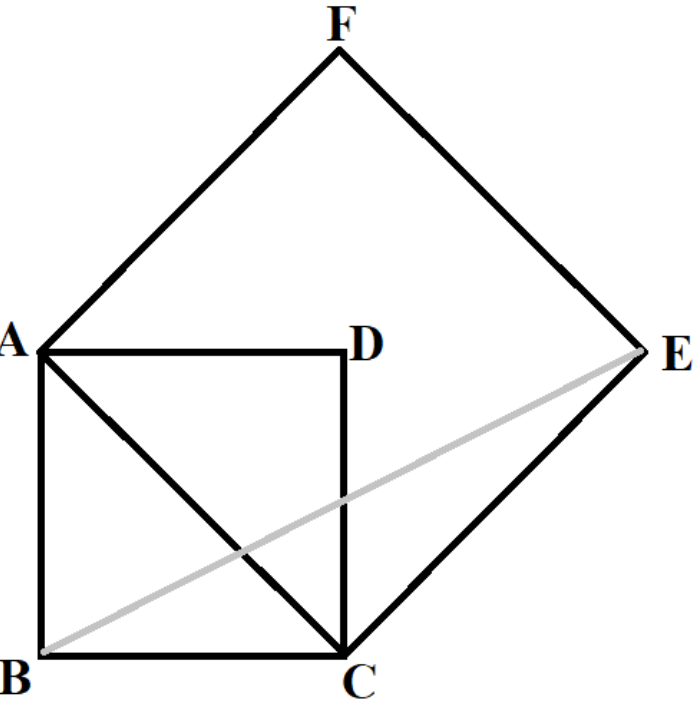
\includegraphics[width=0.2\textwidth]{second.png}
\end{center}


(A) $\sqrt{2}$ (B) $\sqrt{3}$ (C) $\sqrt{5}$ (D) $2\sqrt{2}$ (E) $2\sqrt{3}$
\end{tcolorbox}
\clearpage

\subsection{Problema 6}
\begin{tcolorbox}[statementbox]
Qual o resto da divisão de $113333 + 331111$ por $7$?

(A) 0 (B) 1 (C) 3 (D) 5 (E) 6
\end{tcolorbox}
\clearpage

\subsection{Problema 7}
\begin{tcolorbox}[statementbox]
Uma loja de computadores teve a seguinte ideia pensando na “Black Friday”: no mês de outubro, aumentou o valor dos computadores em $(5p)\%$ em relação a setembro, e no mês de novembro, reduziu o valor dos mesmos em $(4p)\%$ em relação a outubro. Sabe-se que o preço do computador é o mesmo em setembro e novembro (que novidade...). Qual é o valor de $p$?

(a) 5 (B) 8 (C) 10 (D) 12 (E) 15
\end{tcolorbox}
\clearpage

\subsection{Problema 8}
\begin{tcolorbox}[statementbox]
Dizemos que um inteiro positivo é avizinhado se a diferença entre quaisquer dois de seus dígitos consecutivos é sempre igual a $1$. Por exemplo, $123456$, $987654$ e $45656765$ são avizinhados. Quantos são os inteiros entre $500{.}000$ e $600{.}000$ que são avizinhados?

(A) 8 (B) 10 (C) 31 (D) 32 (E) 64
\end{tcolorbox}
\clearpage

\subsection{Problema 9}
\begin{tcolorbox}[statementbox]
De quantas maneiras podemos colocar $5$ garotas em fila, sendo $3$ delas Ana, Beatriz e Carla, de modo que Ana fique entre Beatriz e Carla?

(A) 6 (B) 20 (C) 30 (D) 40 (E) 60
\end{tcolorbox}
\clearpage

\subsection{Problema 10}
\begin{tcolorbox}[statementbox]
Uma cidade euclidiana possui $2$ pontos turísticos $A$ e $B$, ligados por uma linha reta de $420$ metros de comprimento. Ana e Beatriz partem, do ponto $A$, em linha reta, em direção ao ponto $B$, com velocidades constantes de $5$ metros por segundo e $3$ metros por segundo, respectivamente. Enquanto isso, Carla parte do ponto $B$, em linha reta, em direção ao ponto $A$, com velocidade constante de $3$ metros por segundo. Sabendo que as $3$ garotas partem simultaneamente, quanto tempo após a partida Carla estará novamente a uma mesma distância de Ana e Beatriz?

(A) 30 segundos (B) 40 segundos (C) 50 segundos (D) 60 segundos (E) 70 segundos
\end{tcolorbox}
\clearpage

\subsection{Problema 11}
\begin{tcolorbox}[statementbox]
No reticulado a seguir, a distância entre quaisquer dois pontos adjacentes na horizontal ou na vertical é igual a $1$ cm. Qual é a área, em cm$^{2}$, da região hachurada?

  \begin{center}
  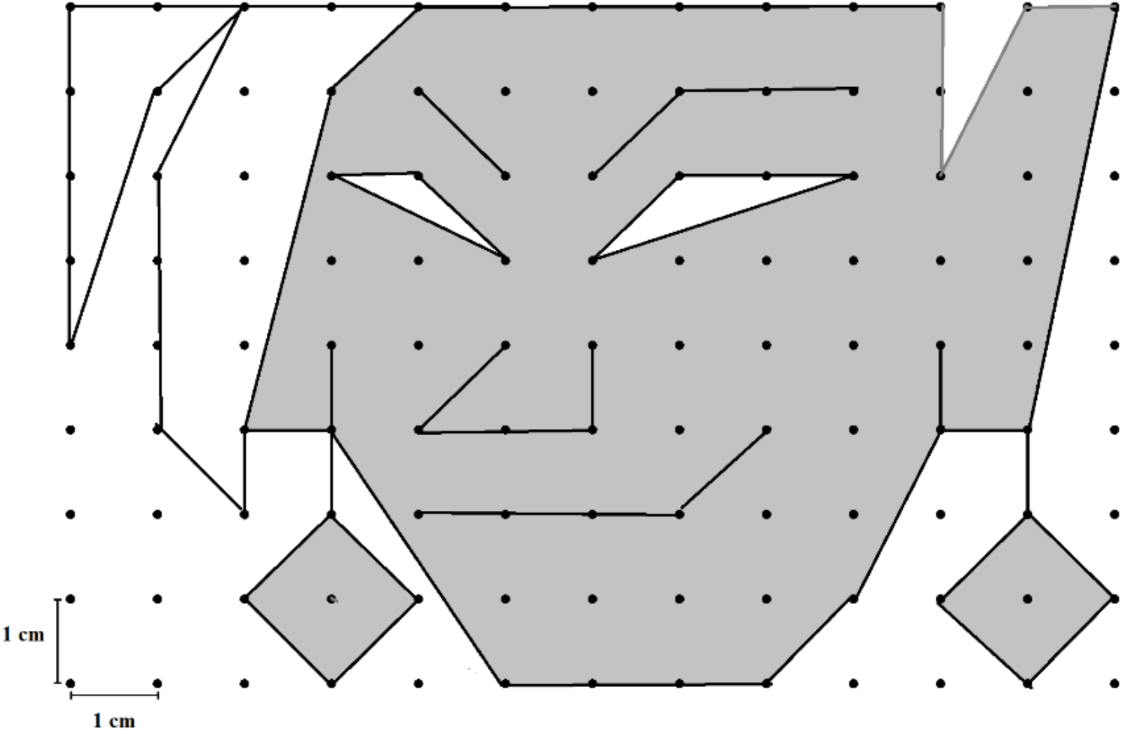
\includegraphics[width=0.5\textwidth]{third.png}
\end{center}


(A) 60 (B) 61 (C) 62 (D) 63 (E) 64
\end{tcolorbox}
\clearpage

\subsection{Problema 12}
\begin{tcolorbox}[statementbox]
Sabe-se que o número $\underbrace{111\ldots 11}_{k\ \text{1’s}}$ é múltiplo de $17$, onde $k$ é um inteiro positivo. Qual é o menor valor possível de $k$?

(A) 4 (B) 11 (C) 16 (D) 18 (E) 34
\end{tcolorbox}
\clearpage

\subsection{Problema 13}
\begin{tcolorbox}[statementbox]
De quantos modos podemos pintar as $5$ regiões da figura abaixo, usando em cada região uma dentre as cores preto, amarelo, rosa, azul e vermelho, de modo que regiões vizinhas tenham cores diferentes? \\
Observação: não é obrigatório que todas as $5$ cores sejam usadas na pintura.


  \begin{center}
  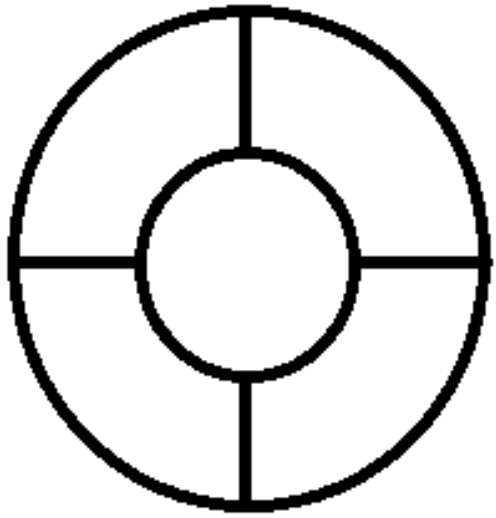
\includegraphics[width=0.25\textwidth]{fourth.png}
\end{center}


(A) 120 (B) 240 (C) 420 (D) 540 (E) 1280
\end{tcolorbox}
\clearpage

\subsection{Problema 14}
\begin{tcolorbox}[statementbox]
Numa sala de aula, a quantidade de meninos é o dobro da quantidade de meninas. Certa vez, foi aplicada uma prova de matemática, e nessa prova a média dos meninos foi $7,4$ enquanto a média das meninas foi $8,6$. Qual foi a média das notas dos alunos da sala?

(A) 7,6 (B) 7,8 (C) 8 (D) 8,2 (E) 8,4
\end{tcolorbox}
\clearpage

\subsection{Problema 15}
\begin{tcolorbox}[statementbox]
No triângulo $ABC$, temos $AB=2AC$. Sejam $D$, $E$ pontos em $\overline{AB}$, $\overline{BC}$, respectivamente, tais que $\angle BAE=\angle ACD$. Seja $F$ a interseção dos segmentos $\overline{AE}$ e $\overline{CD}$, e suponha que o triângulo $CFE$ é equilátero. Qual é a medida do ângulo $\angle ACB$?

(A) $60^\circ$ (B) $75^\circ$ (C) $90^\circ$ (D) $105^\circ$ (E) $120^\circ$
\end{tcolorbox}
\clearpage

\subsection{Problema 16}
\begin{tcolorbox}[statementbox]
Para cada inteiro positivo $n$, sejam: \\
$T_n = 1 + 2 + \cdots + n$ \\
$P_n = \left(\dfrac{T_2}{T_2 - 1}\right)\left(\dfrac{T_3}{T_3 - 1}\right)\cdots\left(\dfrac{T_n}{T_n - 1}\right)$ \\
Qual é a alternativa mais próxima do valor numérico de $P_{2022}$?

(A) 2,90 (B) 2,93 (C) 2,96 (D) 2,99 (E) 3,02
\end{tcolorbox}
\clearpage

\subsection{Problema 17}
\begin{tcolorbox}[statementbox]
Dizemos que um número inteiro é um “Matemático por Diversão” se ele pode ser escrito como a diferença de $2$ quadrados perfeitos não nulos. Por exemplo, $3$ é Matemático por Diversão, pois $3=2^2-1^2$. Quantos são os inteiros positivos, que não excedem $2022$, que são Matemáticos por Diversão?

(A) 506 (B) 507 (C) 1514 (D) 1516 (E) 2020
\end{tcolorbox}
\clearpage

\subsection{Problema 18}
\begin{tcolorbox}[statementbox]
Seja $M=3318084147$. Qual dos números abaixo é um quadrado perfeito?

(A) $M$ (B) $3M$ (C) $5M$ (D) $7M$ (E) $11M$
\end{tcolorbox}
\clearpage

\subsection{Problema 19}
\begin{tcolorbox}[statementbox]
Sejam $x$, $y$ números reais positivos tais que $x^2+y^2=7$ e $x^3+y^3=18$. Quanto vale $x^4+y^4$?

(A) 25 (B) 29 (C) 31 (D) 47 (E) 49
\end{tcolorbox}
\clearpage

\subsection{Problema 20}
\begin{tcolorbox}[statementbox]
Duas circunferências, de raios $3$ e $4$, se cortam em dois pontos, sendo $Q$ um desses pontos. Traçam-se as tangentes externas comuns às duas circunferências. As duas tangentes se cortam em $P$ e uma dessas tangentes tangencia as circunferências nos pontos $A$ e $B$, conforme a figura abaixo: \\
Se $AB=6$, quanto vale $PQ$?

  \begin{center}
  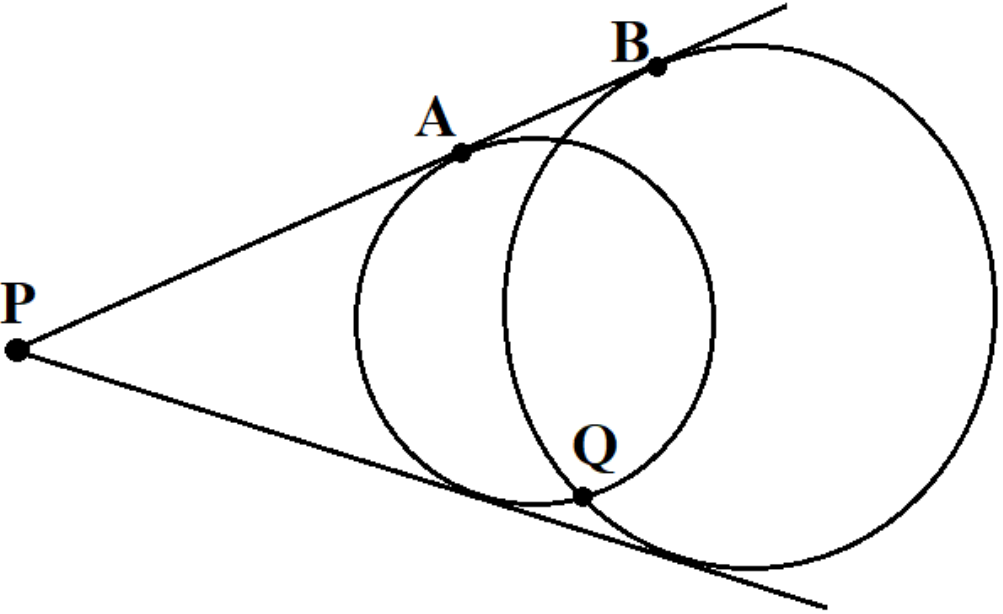
\includegraphics[width=0.25\textwidth]{fifth.png}
\end{center}


(A) 12 (B) $12\sqrt{3}$ (C) 21 (D) $21\sqrt{3}$ (E) 15
\end{tcolorbox}
\clearpage

  \clearpage

  \section{\textsf{Referências}}
\end{document}
